%!TEX TS-program = pdflatex
%!TEX root = main.tex
%!TEX encoding = UTF-8 Unicode



\section{GAN}
Come illustrato nella lezione del MIT \cite{MIT_GEN}, uno tra i primi metodi che ha permesso la generare immagini sintetiche faceva uso di una particolare versione di \emph{Auto-Encoder}(AE), il \emph{Variational Auto-Encoder} (VAE).
Come nel caso degli AE classici, i VAE hanno una struttura che ricorda una clessidra: la prima metà della rete permette di comprimere l'input, mappandolo in quello che viene chiamato spazio latente, di minor dimensione rispetto allo spazio di partenza;  la seconda metà, invece, prende l'input compresso e lo mappa nello spazio di partenza.
Il prodotto della decompressione viene chiamato ``input ricostruito''.
Durante il training si vuole ottimizzare la compressione in modo che non ci sia perdita di informazione, ciò viene effettuato minimizzando la distanza tra input originale ed input ricostruito.
Nei VAE, in corrispondenza del punto della rete in cui si raggiunge il livello massimo di compressione (\emph{bottleneck}), invece di essere generato il vettore compresso $z$, viene prodotta una coppia di vettori $\sigma$ e $\mu$ che descrivono una distribuzione di probabilità dei vettori compressi.
In questo modo è possibile campionare $z$ dalla distribuzione appena prima della decompressione.
Il campionamento non è un'operazione differenziabile e questo rende inapplicabile l'algoritmo della $backpropagation$, quindi risulta necessario effettuare quello che viene chiamato \emph{reparametrization trick}.
Rappresentando $z$ come $z = \mu + \sigma \odot \varepsilon$ in cui $\varepsilon \sim \mathcal{N}(0,1)$, $\varepsilon$ campionata da una distribuzione normale, è possible effettuare l'operazione di \emph{sampling} all'esterno della rete.
In questo modo $\mu$ e $\sigma$ possono essere utilizzati per il calcolo del gradiente e quindi usati durante la \emph{backpropagation}.
Un VAE allenato, poiché ha un \emph{bottleneck} non deterministico, permette di generare immagini con \emph{feature} simili a quelle fornite durante il training, inoltre è possibile modificare direttamente i valori del vettore $z$ per osservare che tipo di informazione rappresentano una volta decompressi.
Nonostante questo tipo di rete sia in grado di dare risultati interessanti e permetta di comprendere meglio il significato degli spazi latenti, è strettamente legata alla dimensions del \emph{bottleneck}.
Quest'ultimo è un \emph{hyperparameter} perché dipende dalla forma della rete, quindi deve essere cercato manualmente.

%Dopo questa breve panoramica sulle VAE, ispirata alla lezione del MIT \cite{MIT_GEN}, ci si accorge che sono una soluzione astuta ma complessa e che le loro prestazioni sono vincolate strettamente allo spazio latente che si è trovato durante il training.

%TODO nota sul Disentanglement delle variabili che permette di avere controllo sulle singole caratteristiche delle immagini generate

Le prestazioni dei VAE sono state superate da quelle dell GAN.
Le \emph{Generative Adversarial Network} (GAN) sono composte da due modelli che, citando \cite{GANTF}, \emph{``vengono addestrati simultaneamente da un processo contraddittorio. Un generatore ("l'artista") impara a creare immagini che sembrano reali, mentre un discriminatore ("il critico d'arte") impara a distinguere le immagini reali dai falsi''}.
Riformulando la frase si può dire che una GAN, come si vede in \autoref{fig:gan}, è composta da due reti: la prima viene chiamata Generatore $G$ ed il suo scopo è fornire in output un $x_{fake}$ che sembri appartenere alla distribuzione del \emph{dataset} di dati reali fornito; la seconda, detta Discriminatore $D$, prende in input un $x_{fake}$ oppure un $x_{real}$ estratto dal \emph{dataset} e deve riuscire determinare se è reale oppure sintetico.
Notare che le GAN non sono strettamente limitate ad immagini, infatti lo scopo dell'architettura è quello di produrre una buona approssimazione della distribuzione di probabilità del dataset attraverso una metrica dinamica determinata da D.
L'idea di partenza è molto semplice però la convergenza del modello non è scontata e sono noti svariati problemi, alcuni dei quali illustrati in \cite{HARD_GAN}.

\begin{figure}[ht]
  \centering
  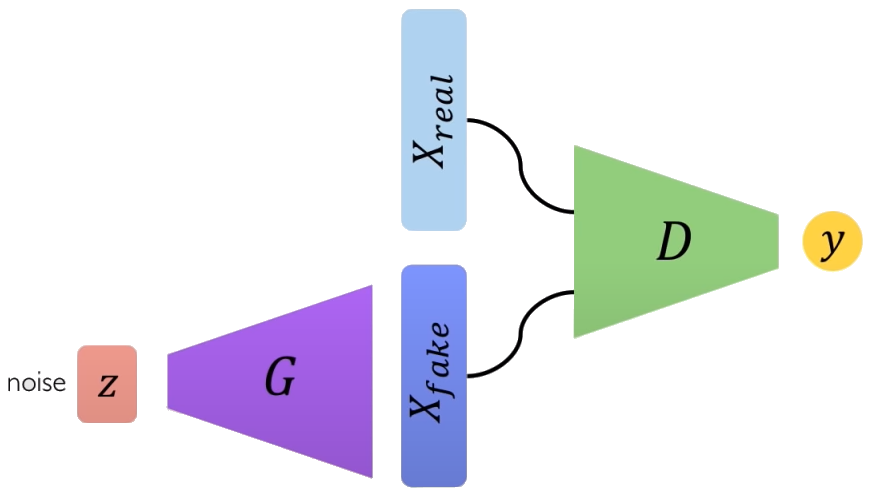
\includegraphics[width=.7\textwidth]{GAN/arch.png}
  \caption{Architettura di una generica GAN (dalle slide in \cite{MIT_GEN})}
  \label{fig:gan}
\end{figure}
\noindent
Il training viene svolto in quattro momenti:
\begin{itemize}
  \item a partire da del rumore casuale $z$, il generatore $G$, basandosi sulle sue conoscenze attuali, produce un $x_{fake}$;
  \item successivamente $D$ riceve un $x_{fake}$ ed un $x_{real}$ e deve categorizzali correttamente;
  \item il \emph{ground truth} è noto, quindi è possibile effettuare la \emph{backpropagation} su $D$;
  \item similmente $G$ viene aggiornato a partire dalla probabilità $D(x_{fake})$ cioè quanto il discriminatore è convinto che $x_{fake}$ sia reale.
    Se questo valore è alto significa che il generatore sta imparando correttamente.
\end{itemize}
Notare come $G$ sia in grado di mappare del rumore casuale nello spazio delle \emph{feature} del dominio e che quindi, una volta allenato, possa essere sfruttato molto facilmente: basterà avere del rumore da cui partire.
In questo senso c'è una certa somiglianza con quanto succede nella seconda parte dei VAE: $G$ opera come un decoder in cui lo spazio latente è molto semplice.

Ci si accorge che $G$ e $D$ hanno obiettivi opposti: il primo vuole confondere il secondo, mentre questo vuole evitare di venire confuso.
Questo gioco di minmax può essere riassunto in  formule con:
$$
min_G \, max_D \: V(D,G) = \E_{x \sim P_{real(x)}} [ log D(x) ] 
+
\E_{z \sim P_z(x)} [ log ( 1 - D(G(z)) ]
$$
$D$ vuole massimizzare il valore atteso della probabilità (in questo caso logaritmica) che un $x$ estratto dal dataset sia effettivamente riconosciuto come reale ed allo stesso tempo vuole massimizzare anche $ 1 - D(x)$ quando $x=G(z)$ è sintetico.
Quindi nel caso del dato reale $D(x)$ dovrà avvicinarsi ad 1, mentre nell'altro caso si vorrà $D(G(z)) \simeq 0$.
Al contempo $G$ vuole minimizzare la formula e, dato che può operare solo sul secondo addendo, tenderà ad indurre $D(G(z)) \simeq 1$.

Rispetto ai $VAE$ le $GAN$ risultano non solo più intuitive ma permettono anche di raggiungere prestazioni veramente sorprendenti, come si può vedere in \cite{GAN_HD}, in cui anche gli esperti umani vengono ingannati dai prodotti della rete.

Va fatto notare però che le GAN sono notoriamente difficili da allenare, come riportato in \cite{HARD_GAN}.
Già ad un livello intuitivo si può capire che partendo da reti senza conoscenze pregresse è molto difficile raggiungere buone prestazioni: entrambe le sotto-reti non hanno alcuna conoscenza del dominio e si chiede loro di guidarsi a vicenda.
Quindi in molte applicazioni, ove possibile, conviene effettuare un \emph{pre-train} dei singoli $G$ e $D$ ed collegarli successivamente per formare l'architettura GAN.
Questo accorgimento comunque non evita un altro problema ben noto: quando il discriminatore converge rapidamente è possibile che dia una valutazione così bassa al generatore da rendere impossibile che $G$ possa migliorarsi.
Quando $D(G(z))$ è pressoché zero si rischia il problema del \emph{vanishing gradient}, quindi i pesi di $G$ vengono aggiranti di un valore troppo piccolo bloccando l'esplorazione dello spazio di ricerca.

Un altro problema difficile da evitare è quello del \emph{model collapse} che si verifica quando $G$ riproduce molto bene soltanto una piccola frazione del dominio.
In questo modo riesce ad ottenere punteggi molto alti a discapito della generalità.
A seconda del dominio di applicazione il \emph{model collapse} può essere un problema più o meno grave e richiedere accorgimenti specifici.
Un caso particolare che preclude la convergenza della GAN si ha quando $G$ si specializza per confondere $D$ in un modo specifico, poi $D$ si aggiorna per difendersi contro quel modo specifico, a quel punto $G$ si specializza su un ulteriore modo specifico.
Se i modelli continuano questo ``inseguimento'' non convergeranno mai ad una soluzione utile.

% alcuni modi per risolvere model collapse?


% L'efficacia di questa tecnica e' lampante quando si parla di immagini...
%In questo caso si fa riferimento alla possibilità di utilizzare le GAN come generatori di immagini sintetiche indistinguibili da quelle reali, in \cite{GAN_HD} si può osservare il livello di dettaglio impressionante che queste reti sono in grado di produrre.


%\todo[inline]{aggiungere robe dal paper originale se si deve allungare}

